\subsection{Summary of the Exoplanet Catalog}
The DR25 exoplanet candidate catalog has the following properties:
\begin{itemize}
    \item [o] plot of pradius vs. period and/or pradius vs insol. flux
    \item [o] Histogram of number of candidates of different sizes (short and long period)
    \item [o] Discuss number of candidates compared to previous catalogs.
    \item [o] Discuss identified EBs.
    \item [o] From looking at distributions obvious over abundance at 370 days.
\end{itemize}

\begin{figure*}
    \centering
    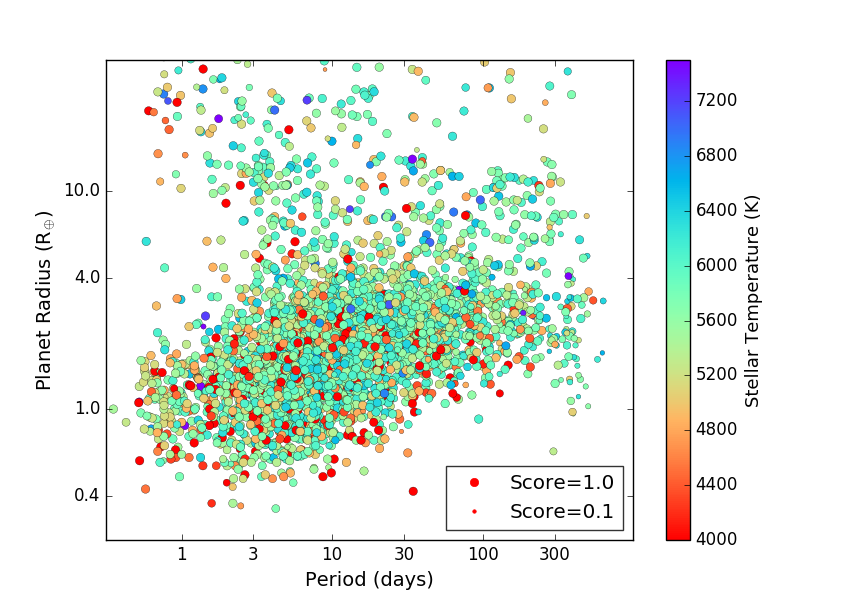
\includegraphics[width=1.1\linewidth]{fig-CatalogRadiusPeriodScore.png}
    \caption{DR25 Exoplanet Candidates plotted as planet radius against Period. The stellar temperature is given by the color of the circle and the size of the circle indicates the Disposition Score. The planet radii are derived from the MCMC fits. }
    \label{f:catalogPlot}
\end{figure*}